% Ubah judul dan label berikut sesuai dengan yang diinginkan.
\section{Parity Bit}
\label{sec:paritybit}

% Ubah paragraf-paragraf pada bagian ini sesuai dengan yang diinginkan.

Pada ilmu Matematika, paritas merupakan sebuah properti dari sebuah \emph{integer} yang menentukan apabila \emph{integer} tersebut ganjil atau genap. Sebuah paritas dari bilangan bulat adalah genap apabila jika bilangan tersebut dapat dibagi dengan dua dan sisanya adalah nol. Sebaliknya jika sisanya satu maka paritasnya adalah ganjil.
\emph{Parity Bit} atau biasa juga disebut dengan \emph{Check Bit} adalah bentuk sederhana dari \emph{error detecting code}. Error detecting code ini biasa digunakan untuk melakukan transmisi digital data yang \emph{reliable} dengan menggunakan kanal komunikasi yang \emph{unreliable}. Semua bentuk error detection akan menambahkan beberapa data ekstra pada pesan, yang dapat digunakan oleh penerima untuk melakukan verifikasi dari konsitensi pada pesan tersebut. \emph{Parity bit} akan memastikan bahwa jumlah total dari 1-bit pada sebuah string adalah ganjil atau genap \citep{rodger2015}.

Terdapat dua varian dari bit paritas, paritas genap dan paritas ganjil. Pada kasus paritas genap, untuk setiap bit dari string yang diberikan, jumlah bit yang bernilai 1 akan dihitung. Apabila jumlahnya ganjil, maka nilai dari bit paritas akan diatur menjadi 1, yang membuat total bit 1 menjadi bernilai genap. Sebaliknya, jika jumlah dari bit 1 pada awalnya sudah genap, maka bit paritas akan diatur menjadi 0. Pada kasus paritas ganjil, prosedurnya akan berkebalikan. Untuk setiap bit dari string yang diberikan, jumlah bit yang bernilai 1 akan dihitung. Apabila jumlahnya genap, maka nilai dari bit paritas akan diatur menjadi 1, yang membuat total bit 1 menjadi bernilai ganjil. Sebaliknya, jika jumlah dari bit 1 pada awalnya sudah ganjil, maka bit paritas akan diatur menjadi 0.

\begin{figure} [ht]
  \centering
  % Ubah sesuai dengan nama file gambar dan ukuran yang akan digunakan.
  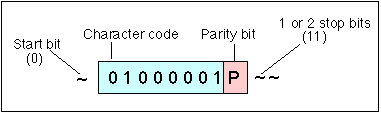
\includegraphics[width=0.4\textwidth]{gambar/parity.png}

  % Ubah sesuai dengan keterangan gambar yang diinginkan.
  \caption{Struktur parity bit}
  \label{fig:parityexample}
\end{figure}

% Contoh pembuatan tabel.
\begin{table}
  \caption{Contoh bit paritas}
  \label{tab:parityexample}
  \centering
  \rowcolors{3}{green!80!yellow!50}{green!70!yellow!40}
  \begin{tabular}{cccc}
    \toprule
    & & \multicolumn{2}{c}{8 bits including parity} \\
    7 bits of data & Count of 1 bits & even & odd \\
    \midrule
    0000000        & 0               & 00000000 & 00000001 \\
    1010001        & 3               & 10100011 & 10100010 \\
    1101001        & 4               & 11010010 & 11010011 \\
    1111111        & 7               & 11111111 & 11111110 \\
    \bottomrule
  \end{tabular}
\end{table}

Apabila sebuah string yang berisi bit-bit paritas ditransmisikan secara tidak benar atau korup, maka bit paritasnya akan salah. Hal tersebut mengindikasikan terjadinya \emph{parity error} saat transmisi. Bit paritas ini hanya bisa mendeteksi adanya error; tidak dapat melakukan koreksi error pada file yang terjadi, karena tidak ada mekanisme yang memungkinkan bit paritas untuk mengetahui bit yang mana yang korup. Lalu apabila meninjau Tabel \ref{tab:parityexample}, dapat diketahui bahwa bit paritas ini memiliki kelemahan. Bit paritas hanya mengecek jumlah bit ganjil atau genap tanpa meninjau jumlah asli bitnya. Hal ini mengakibatkan terjadinya kegagalan dalam menangkap error pada data. Sebagai contoh, jika A ingin mengirim data \verb|1001| dengan paritas genap maka bit paritasnya adalah \verb|0| sehingga yang ditransmisikan ke B adalah \verb|10010|. Terjadi error pada transmisi, sehingga yang sampai ke B adalah \verb|11011|. Akan tetapi, B menghitung jumlah bit dan mendapati genap, sehingga B akan menganggap data tersebut benar walaupun sebenarnya salah.

% Contoh input potongan kode dari file.
\lstinputlisting[
  language=Python,
  caption={Program perhitungan bit paritas genap.},
  label={lst:paritasgenap}
]{program/paritas_genap.py}

\begin{lstlisting}[
  language=Python,
  caption={Program perhitungan bit paritas ganjil},
  label={lst:paritasganjil}
]
def odd_parity(x):
    parity = 1
    while x:
        parity ^= x & 1
        x >>= 1
    return parity
\end{lstlisting}

Potongan kode pada Listing \ref{lst:paritasgenap} diatas adalah contoh kode yang berfungsi menemukan bit paritas genap. Untuk bit paritas ganjil tinggal mengganti inisialisasi variabel parity menjadi 1. Inputnya adalah \emph{integer} yang bisa kita jadikan biner dulu, seperti \verb|0b10001|.

% % Contoh pembuatan persamaan ilmiah.
% \begin{equation}
%   \label{eq:hukumpertama}
%   \sum \mathbf{F} = 0\; \Leftrightarrow\; \frac{\mathrm{d} \mathbf{v} }{\mathrm{d}t} = 0.
% \end{equation}
